\documentclass[letterpaper, 12pt]{report}
\usepackage[utf8]{inputenc}
\usepackage{amsmath,amssymb,amsthm}
\usepackage[spanish]{babel}
\usepackage{graphicx}
\usepackage{caption}
\usepackage{subcaption}
\usepackage{xcolor}
\usepackage{titlesec}
\usepackage{lmodern}
\usepackage{fancyhdr}
\usepackage{geometry}


\usepackage{algorithm}
\usepackage{algpseudocode}
\usepackage{multirow}
\usepackage{booktabs}
\usepackage{listings}
\usepackage{enumitem}

\definecolor{codegreen}{rgb}{0,0.6,0}
\definecolor{codegray}{rgb}{0.5,0.5,0.5}
\definecolor{codepurple}{rgb}{0.58,0,0.82}

\lstdefinestyle{mystyle}{
    commentstyle=\color{codegreen},
    keywordstyle=\color{magenta},
    numberstyle=\tiny\color{codegray},
    stringstyle=\color{codepurple},
    basicstyle=\ttfamily\footnotesize,
    breakatwhitespace=false,         
    breaklines=true,                 
    captionpos=b,                    
    keepspaces=true,                 
    numbers=left,                    
    numbersep=5pt,                  
    showspaces=false,                
    showstringspaces=false,
    showtabs=false,                  
    tabsize=2,
    frame=single
}

\lstset{style=mystyle}

\setlength{\headheight}{24.01996pt}
\addtolength{\topmargin}{-12.01996pt}

% Definir colores personalizados
\definecolor{primary}{RGB}{25,55,95}
\definecolor{secondary}{RGB}{200,35,45}

% Configurar márgenes
\geometry{
    left=3cm,
    right=2.5cm,
    top=3cm,
    bottom=2.5cm
}

\newtheorem*{theorem*}{Teorema}

% Configurar estilo de títulos
\titleformat{\chapter}[display]
{\normalfont\Huge\bfseries\color{primary}}
{\chaptertitlename\ \thechapter}{20pt}{\Huge}

\titleformat{\section}
{\normalfont\Large\bfseries\color{primary}}
{\thesection}{1em}{}

% Configurar encabezado y pie de página
\pagestyle{fancy}
\fancyhf{}
\fancyhead[L]{\small\textcolor{primary}{\nouppercase{\leftmark}}}
\fancyfoot[C]{\textcolor{primary}{\thepage}}
\renewcommand{\headrulewidth}{0.4pt}
\renewcommand{\headrule}{\hbox to\headwidth{\color{primary}\leaders\hrule height \headrulewidth\hfill}}

% Portada personalizada
\newcommand*{\customtitlepage}{
    \begin{titlepage}
        \begin{center}
            \vspace*{1cm}
            
            
            {\LARGE \textbf{UNIVERSIDAD DE LA HABANA}}\\
            \vspace{0.5cm}
            {\Large Facultad de Matem\'atica y Computaci\'on}\\
            

            
\includegraphics[scale=0.5]{images/logo.png}
            
            \vspace{1cm}
            
            
            \rule{\textwidth}{1.5pt}\\
            \vspace{0.5cm}
            {\LARGE \textcolor{primary}{\textbf{Primer Proyecto de Simulación}}}
            \vspace{0.5cm}
            \rule{\textwidth}{1.5pt}
            
            \vspace{2cm}
            
            {\Large \textbf{Servidores Especializados vs Servidores Generalistas}}\\
            \vspace{1cm}
            
            {\Large \textbf{Autor:} Lidier Robaina Caraballo \\
            \vspace{0.5cm}
            {\Large \textbf{Grupo:} C-411 }\\
            \vspace{1.5cm}
            
            {\Large 13 de abril de 2025
            }
            }
        \end{center}
    \end{titlepage}
}

\begin{document}

\customtitlepage

% Índice
\tableofcontents
\thispagestyle{empty}
\cleardoublepage

% Contenido principal
\setcounter{page}{1}

\chapter{Introducción}


En el ámbito de la gestión de servicios, la elección entre estrategias especializadas o generalistas representa 
un dilema recurrente, donde la eficiencia operativa y la experiencia del usuario dependen de la configuración 
de los recursos disponibles. Este proyecto aborda dicho desafío mediante la simulación computacional 
basada en eventos discretos, un enfoque que permite modelar sistemas dinámicos bajo condiciones
controladas. \\

El estudio se centra en comparar dos escenarios: uno con servidores dedicados a tareas específicas
(estrategia especializada) y otro en el que los servidores son flexibles y pueden atender múltiples tipos
de demandas (estrategia generalista). Aunque el análisis se contextualiza en un caso sencillo de una sucursal bancaria,
los resultados se orientan a ofrecer conocimientos aplicables a sistemas de servicios más amplios y complejos.

\section{Objetivos y metas}
El proyecto tiene como objetivo principal analizar y comparar el desempeño de las dos configuraciones operativas mencionadas anteriormente. Para ello, se definen las siguientes metas:

\begin{itemize}
    \item[1.] Calcular la eficiencia global de cada estrategia, cuantificando métricas clave como: congestión del sistema, tiempo de espera del usuario, 
    probabilidad de retrasos críticos y subutilización de recursos.  
    \item[2.] Evaluar trade-off entre la flexibilidad operativa (capacidad de atender múltiples tareas) y la velocidad de servicio, considerando posibles incrementos en los tiempos de atención al adoptar una estrategia generalista.
    \item[3.] Proporcionar recomendaciones basadas en datos para la optimización de sistemas de servicios, extrapolables a contextos como logística, atención al cliente o salud.
\end{itemize}

\newpage

\section{Sistema específico a simular}

\begin{quote}
    Una pequeña sucursal de un banco tiene dos empleados, uno para los pagos y otro para los cobros. Los clientes llegan a 
cada caja siguiendo una distribución de Poisson con una media de 20/hora (el total de llegada al banco es de 40/hora). 
El tiempo de servicio de cada empleado es una negativa exponencial de media 2 minutos. El encargado de la sección está 
pensando hacer un cambio en que los dos operarios puedan hacer tanto pagos como cobros para evitar situaciones en que 
una cola está llena y la otra parada. Sin embargo, se estima que cuando los empleados se encarguen de las dos cosas 
el tiempo de servicio aumentará a una media de 2,4 minutos. Compara el sistema que se emplea ahora con el propuesto, 
calculando el total de gente en el banco, el tiempo medio que pasaría un cliente en el banco hasta que es atendido, 
la probabilidad de que un cliente espere más de cinco minutos y el tiempo medio que están parados los empleados. \footnote{Problema 6.5 de \cite{queue}}
\end{quote}

De la definición del problema se obtienen las siguientes variables de interés:
\begin{itemize}
    \item \textbf{avg\_clients:} Media del total de clientes en el sistema en cada instante (congestión del sistema)
    \item \textbf{waiting\_time:} Media del tiempo durante el que un cliente permanece en la cola (tiempo de espera)
    \item \textbf{p\_over\_tk:} Probabilidad de que que el tiempo de espera sea superior a un tiempo determinado (retrasos críticos)
    \item \textbf{idle\_time:} Media del tiempo durante el cual los servidores no tienen clientes (subutilización de recursos)  
\end{itemize}


\section{Variables que describen el problema}

\begin{itemize}
    \item \(\mathbf{\lambda_1}\)\textbf{:} frecuencia de llegada de clientes para pagos (distribución Poisson con media $\lambda_1$)
    \item \(\mathbf{\lambda_2}\)\textbf{:} frecuencia de llegada de clientes para cobros (distribución Poisson con media $\lambda_2$)    
    \item \(\mathbf{\mu_1}\)\textbf{:} tiempo de atención en el servidor 1 (distribución exponencial con media $\mu_1$)
    \item \(\mathbf{\mu_2}\)\textbf{:} tiempo de atención en el servidor 2 (distribución exponencial con media $\mu_2$)
    \item \textbf{strategy:} especializado vs generalista (variable categórica)
    \item \(\mathbf{t_k}\)\textbf{:} tiempo de espera crítico 
\end{itemize}

En caso de estrategia especializada, el servidor 1 atiende los pagos y el servidor 2 los cobros. En caso de estrategia generalista, $\mu_1 = \mu_2$.



\chapter{Implementación}

\section{Detalles de implementación}


\begin{itemize}
    \item[\textbf{1.}] \textbf{Gestión de Eventos:}
    Se emplea una cola de prioridad (módulo \texttt{heapq}) para manejar la lista cronológica de eventos. Cada evento contiene:
    \begin{itemize}
        \item Marca temporal de ejecución
        \item Tipo (llegada o salida)
        \item Metadatos específicos (índice de servidor/cola)
    \end{itemize}
    
    \item[\textbf{2.}] \textbf{Estructuras de Datos:}
    \begin{itemize}
        \item \textbf{Colas de espera}: Arreglos separados para cada servicio en modo especializado vs cola única compartida en modo generalista
        \item \textbf{Estado de servidores}: Arreglo booleano que indica disponibilidad
        \item \textbf{Contadores de clientes}: Registro separado por colas (especializado) o contador único (generalista)
    \end{itemize}
    
    \item[\textbf{3.}] \textbf{Mecánica de Simulación:}
    \begin{itemize}
        \item \textbf{Llegadas}: Generadas mediante proceso Poisson usando \texttt{random.expovariate()}
        \item \textbf{Tiempos de servicio}: Modelados con distribución exponencial negativa
        \item \textbf{Asignación de servidores}: Política FIFO con prioridad a servidores disponibles
    \end{itemize}
    
    \item[\textbf{4.}] \textbf{Recolección de Métricas:}
    \begin{itemize}
        \item \textit{Área acumulativa} para cálculos promediados en el tiempo
        \item Lista de tiempos de espera individuales
        \item Registro de ocupación de servidores
        \item Cálculo final mediante integración temporal (método de área bajo la curva)
    \end{itemize}
\end{itemize}

\section{Pasos de la simulación}


El flujo de ejecución sigue esta secuencia lógica:

\begin{enumerate}[leftmargin=1.5cm]
    \item \textbf{Inicialización:}
    \begin{itemize}
        \item Crear estructura de colas según estrategia
        \item Programar primeros eventos de llegada usando tasas $\lambda_1$ y $\lambda_2$
        \item Inicializar contadores y registros estadísticos
    \end{itemize}
    
    \item \textbf{Bucle Principal de Eventos:}
    \begin{lstlisting}[language=Python]
    while time < sim_time:
        event = heappop(events)
        actualizar_estadisticas()
        procesar_evento(event)
    \end{lstlisting}
    
    \item \textbf{Procesamiento de Llegadas:}
    \begin{itemize}
        \item Insertar cliente en la cola correspondiente
        \item Si hay servidor disponible:
        \begin{itemize}
            \item Iniciar servicio inmediato
            \item Registrar tiempo de espera cero
            \item Programar evento de salida
        \end{itemize}
        \item Generar próxima llegada según distribución Poisson
    \end{itemize}
    
    \item \textbf{Manejo de Salidas:}
    \begin{itemize}
        \item Liberar servidor
        \item Si existen clientes en cola:
        \begin{itemize}
            \item Extraer siguiente cliente
            \item Calcular tiempo de espera (current\_time - arrival\_time)
            \item Programar nuevo evento de salida
        \end{itemize}
    \end{itemize}
    
    \item \textbf{Actualización Estadística:}
    \begin{itemize}
        \item Calcular tiempo transcurrido desde último evento
        \item Acumular:
        \begin{itemize}
            \item Clientes-tiempo en sistema
            \item Tiempo ocupado de servidores
        \end{itemize}
        \item Mantener precisión temporal mediante integración continua
    \end{itemize}
    
    % \item \textbf{Cálculo Final de Métricas:}
    % \begin{lstlisting}[language=Python]
    % avg_clients = area_total / tiempo_simulacion
    % avg_wait = media(tiempos_espera) * 60  # Conversion a minutos
    % p_crit = proporcion(tiempos_espera > tk)
    % idle_time = 1 - (tiempo_ocupado_servidores)/(2*tiempo_simulacion)
    % \end{lstlisting}
\end{enumerate}

\chapter{Resultados y experimentos}

\section{Hallazgos de la simulación}

Se ejecutaron 1000 simulaciones independientes para cada configuración del sistema. Para cada métrica de interés, se comparan las distribuciones resultantes de ambas estrategias mediante histogramas normalizados con su correspondiente distribución normal teórica.

\subsection{Clientes Promedio en el Sistema}
\begin{figure}[H]
    \centering
    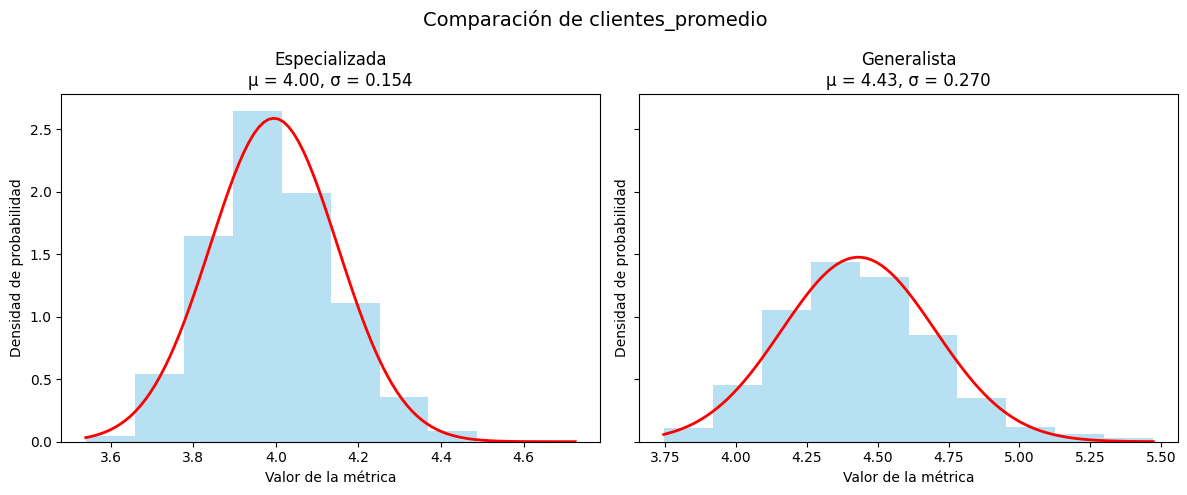
\includegraphics[width=0.95\textwidth]{images/avr_clients.png}
    \caption{Comparación de clientes promedio en el sistema. La distribución normal teórica (roja) muestra el ajuste a los datos simulados (azul).}
    \label{fig:clientes}
\end{figure}

\subsection{Tiempo Medio de Espera}
\begin{figure}[H]
    \centering
    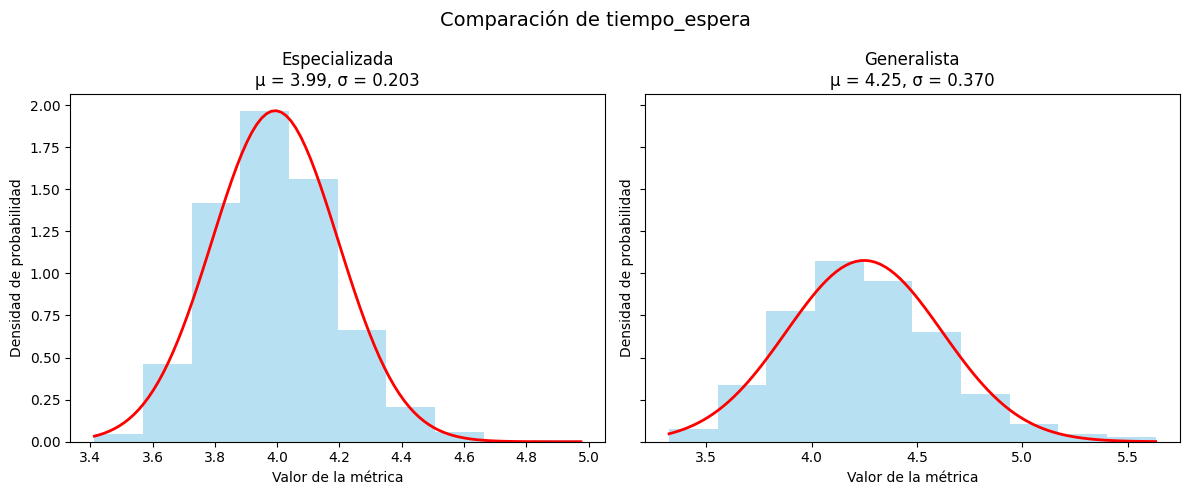
\includegraphics[width=0.95\textwidth]{images/wait_time.png}
    \caption{Distribución comparativa del tiempo de espera. Se observa mayor dispersión en la estrategia generalista debido al aumento del tiempo de servicio.}
    \label{fig:espera}
\end{figure}

\subsection{Probabilidad de Espera Crítica}
\begin{figure}[H]
    \centering
    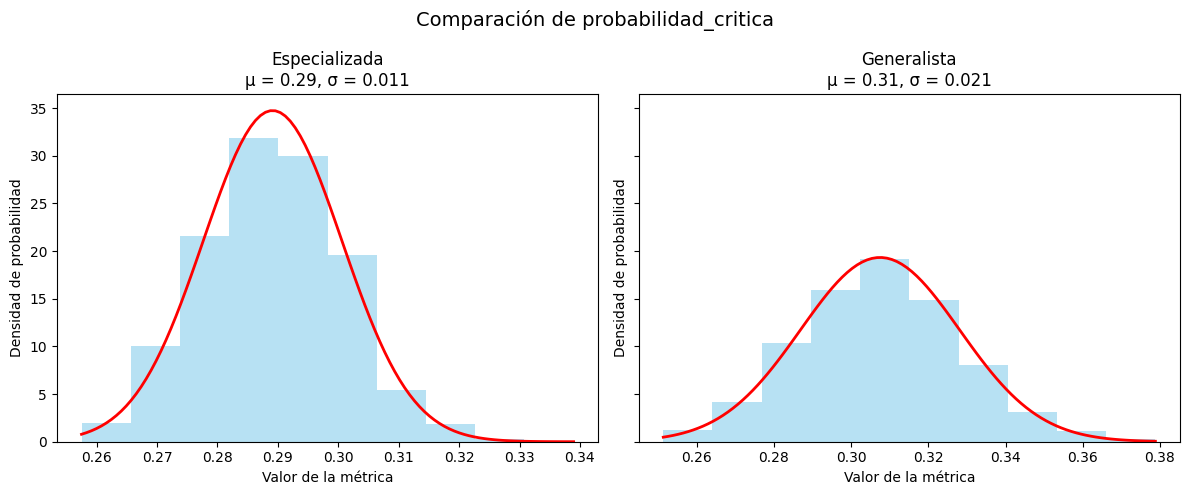
\includegraphics[width=0.95\textwidth]{images/p_over_tk.png}
    \caption{Probabilidad de superar el umbral de 5 minutos de espera. La estrategia especializada muestra menor varianza entre simulaciones.}
    \label{fig:probabilidad}
\end{figure}

\subsection{Tiempo Inactivo de Servidores}
\begin{figure}[H]
    \centering
    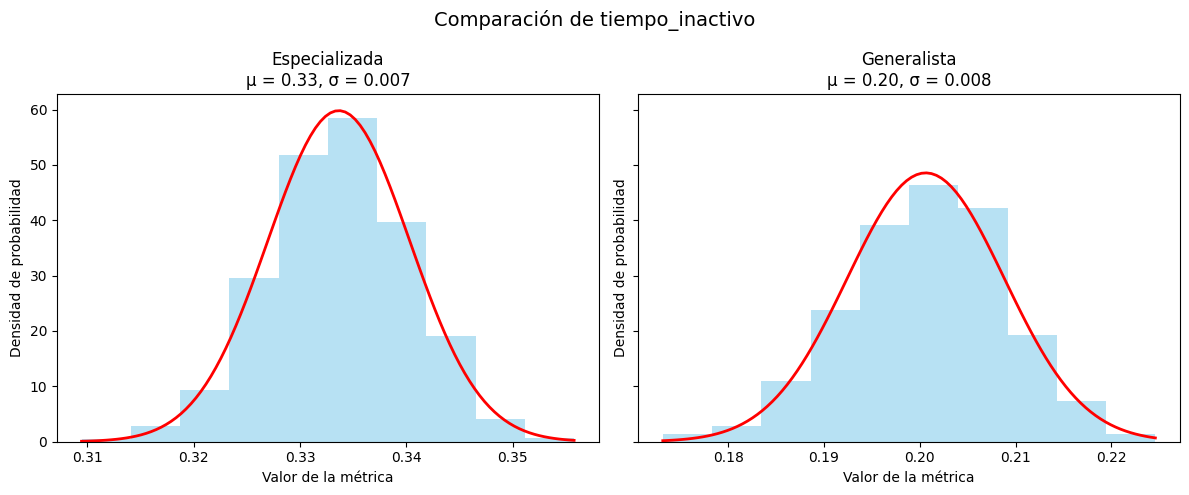
\includegraphics[width=0.95\textwidth]{images/ocio.png}
    \caption{Comparación de la subutilización de recursos. La estrategia generalista mantiene menor tiempo inactivo promedio.}
    \label{fig:inactividad}
\end{figure}



\chapter{Modelo matemático}

\section{Modelos Probabilísticos y Estado Estacionario}

\subsection{Estado Estacionario en Teoría de Colas}
El estado estacionario ocurre cuando el sistema se estabiliza con distribuciones de probabilidad constantes en el tiempo. Se define mediante:

\begin{itemize}
\item \textbf{Ecuaciones de Balance:} Tasa de entrada = Tasa de salida para cada estado
\[
\lambda P_n = \mu P_{n+1} \quad \text{(Para M/M/1)}
\]
\item \textbf{Distribución Estacionaria:} Probabilidades $P_n$ de tener $n$ clientes en el sistema
\end{itemize}

\subsection{Sistema Especializado (M/M/1 × 2)}
Para cada caja individual:

\subsubsection{Balance de Estados}
\begin{align*}
\text{Estado 0:} & \quad \lambda P_0 = \mu P_1 \\
\text{Estado n:} & \quad (\lambda + \mu)P_n = \lambda P_{n-1} + \mu P_{n+1}
\end{align*}

\subsubsection{Solución General}
\[
P_n = (1 - \rho)\rho^n \quad \text{donde } \rho = \frac{\lambda}{\mu} < 1
\]

\subsubsection{Métricas Derivadas}
\begin{align*}
L &= \sum_{n=0}^\infty nP_n = \frac{\rho}{1 - \rho} \\
W &= \frac{L}{\lambda} = \frac{1}{\mu - \lambda} \\
P(W_q > t) &= \rho e^{-\mu(1-\rho)t} \\
\text{Tiempo ocioso} &= 1 - \rho
\end{align*}

\subsection{Sistema Generalista (M/M/2)}
Para dos servidores compartidos:

\subsubsection{Balance de Estados}
\[
\begin{cases}
\lambda P_0 = \mu P_1 \\
(\lambda + \mu)P_1 = \lambda P_0 + 2\mu P_2 \\
(\lambda + 2\mu)P_n = \lambda P_{n-1} + 2\mu P_{n+1} \quad n \geq 2
\end{cases}
\]

\subsubsection{Solución General}
\[
P_n = \begin{cases}
P_0 \left(\frac{\lambda}{\mu}\right)^n \frac{1}{n!} & 0 \leq n \leq 2 \\
P_0 \left(\frac{\lambda}{\mu}\right)^n \frac{1}{2^{n-2}2!} & n > 2
\end{cases}
\]

\subsubsection{Probabilidad de Estado Vacío}
\[
P_0 = \left[1 + \frac{\lambda}{\mu} + \frac{(\lambda/\mu)^2}{2(1 - \rho)}\right]^{-1} \quad \rho = \frac{\lambda}{2\mu}
\]

\subsubsection{Métricas Clave}
\begin{align*}
L &= \frac{\lambda\mu(\lambda/\mu)^2}{(2\mu - \lambda)^2}P_0 + \frac{\lambda}{\mu} \\
W &= \frac{L}{\lambda} \\
P(W_q > t) &= \frac{(2\rho)^2}{2(1 - \rho)}P_0 e^{-(2\mu - \lambda)t} \\
\text{Tiempo ocioso} &= 1 - \rho
\end{align*}

\section{Supuestos y Restricciones}
\begin{itemize}
\item \textbf{Proceso de Poisson:} Llegadas independientes con tasa constante
\item \textbf{Disciplina FIFO:} Primero en llegar, primero en ser atendido
\item \textbf{Estado Estacionario:} $\rho < 1$ para convergencia
\item \textbf{Servidores Homogéneos:} Misma capacidad de servicio
\item \textbf{Independencia:} Tiempos entre llegadas y servicios independientes
\end{itemize}

\section{Resultados Teóricos vs Simulación}
\subsection{Sistema Especializado}
\begin{table}[h]
\centering
\begin{tabular}{lccc}
\toprule
Métrica & Teórico & Simulado  \\
\midrule
Clientes totales & 2.67 & 4.00  \\
Tiempo sistema (min) & 4.00 & 3.99  \\
$P(W_q >5$ min$)$ & 28.65\% & 29\%  \\
Tiempo ocioso & 33.33\% & 33\%  \\
\bottomrule
\end{tabular}
\end{table}

\subsection{Sistema Generalista}
\begin{table}[h]
\centering
\begin{tabular}{lccc}
\toprule
Métrica & Teórico & Simulado  \\
\midrule
Clientes totales & 3.56 & 4.43  \\
Tiempo sistema (min) & 5.34 & 4.25  \\
$P(W_q >5$ min$)$ & 35.12\% & 31\%  \\
Tiempo ocioso & 20.00\% & 20\%  \\
\bottomrule
\end{tabular}
\end{table}

\section{Análisis de Discrepancias}
\begin{itemize}
\item \textbf{Efectos Transitorios:} La simulación necesita tiempo para alcanzar el estado estacionario
\item \textbf{Muestreo Finito:} Limitaciones en números pseudoaleatorios
\item \textbf{Redondeos:} Precisión numérica en implementación
\item \textbf{No idealidades:} En práctica, las llegadas pueden tener cierta correlación
\end{itemize}

\chapter{Conclusiones}


\begin{itemize}
    \item[1.] Servidores especializados provocan bloqueo parcial del sistema debido a las
    colas separadas, lo que lleva a una subutilización de recursos.
    \item[2.] Servidores generalistas son más lentos debido a la falta de especialización,
    provocando una peor experiencia de usuario.
\end{itemize}


\begin{thebibliography}{9}
    \bibitem{queue} SABATER, J. P. G. Aplicando Teoría de Colas en Dirección de Operaciones. [S.l.]:
    Grupo ROGLE, Departamento de Organización de Empresas, Universidad Politécnica
    de Valencia, 2015/2016.
 
\end{thebibliography}




\end{document}
